
\section{Algunas propiedades}

\subsection{Desigualdad de Jensen}
Sea la función convexa $f(S)$ (que se curva hacia arriba, con forma de cuenco) de la variable aleatoria $S$, entonces
\[\mathbb{E}[f(S)] \geq f(\mathbb{E}[S])\]
De hecho, la diferencia es de
\[\frac{1}{2}f''(\mathbb{E}[S])\mathbb{E}[\epsilon]\]
donde $\epsilon$ es la desviación de $S$ de la media, i.e $S=\mathbb{E}[S]+\epsilon$.


\subsection{Propiedad de Markov}
\textit{El futuro depende solo del presente, no del pasado.} Se usa en los caminos aleatorios para decir que el valor $S_t+1$ solo depende de $S_t$, es decir,
\[\mathbb{P}(X_{t+s} \in A \mid X_t = x, X_{t_1} = x_1, \ldots, X_{t_n} = x_n) 
= \mathbb{P}(X_{t+s} \in A \mid X_t = x)\]



\subsection{Propiedad de martingala}
\textit{Lo que esperas tener en el futuro, sabiendo todo hasta ahora, es exactamente lo que tienes ahora}. Es decir, el valor esperado de algo en un juego justo es exactamente lo que tienes ahora:
\[\mathbb{E}[S_i|S_j, j<i]=S_j\]



\subsection{Lema de Itô}
Sea
\[dS = a(S,t)dt + b(S,t)d\mathnormal{X}\]
entonces
\begin{equation}
    \boxed{dV = \left( \frac{dV}{dt} +  a\frac{dV}{dS} + \frac{1}{2}b^2\frac{d^2V}{dS^2} \right)dt + b\frac{dV}{dS}d\mathnormal{X}}
\end{equation}\label{Ito}
En el apéndice~\ref{CalcIto} se encuentra la fórmula para dimensiones mayores.

\subsection{Algunos ejemplos de caminos aleatorios}

\begin{itemize}
    \item \textbf{Brownian Motion with Drift}: $\boxed{dS = \mu dt + \sigma d\mathnormal{X}}$
    \begin{figure}[H]
        \centering
        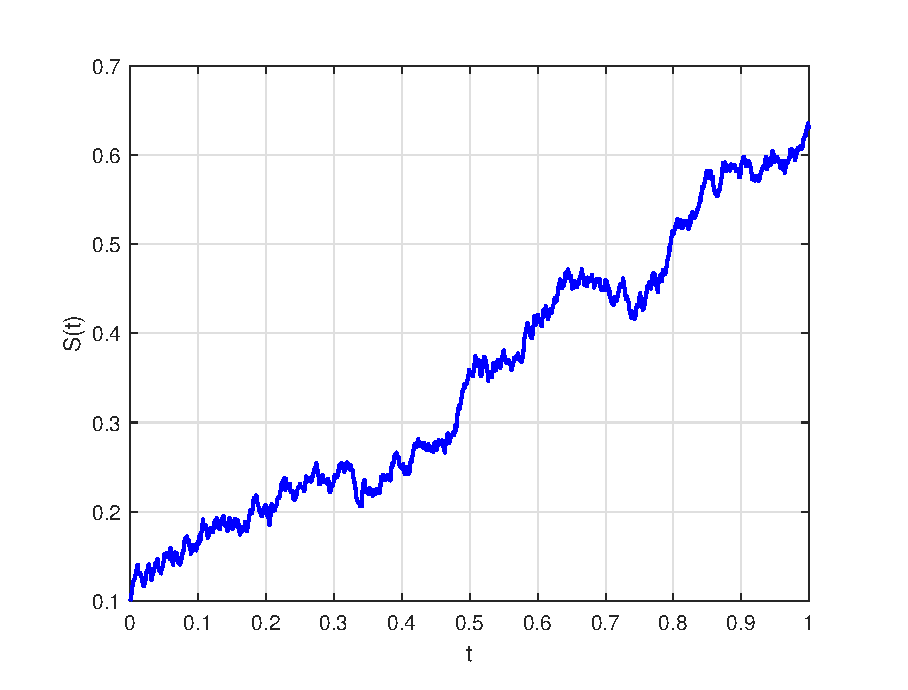
\includegraphics[width=0.65\linewidth]{Imagenes/Parte1/3_Aleatoriedad/BrownianMotionDrift.eps}
        \caption{Brownian Motion with Drift}
    \end{figure}
    \item \textbf{The Lognormal Random Walk}: $\boxed{dS = S\mu dt + S\sigma d\mathnormal{X}}$
    \begin{figure}[H]
        \centering
        \includegraphics[width=0.65\linewidth]{Imagenes/Parte1/3_Aleatoriedad/LognormalRandomWalk.eps}
        \caption{The Lognormal Random Walk}
    \end{figure}
    \item \textbf{A Mean-reverting Random Walk}: reversion a la media, cuando se esta fuera del crecimiento normal el camino tiende a corregirse.\\
    Su EDE es 
    \[
        \boxed{dS = \kappa(\theta+S) dt + \sigma d\mathnormal{X}}
    \]
    donde $\kappa$ es la velocidad de reversión a la media, $\theta$ es la tasa de interés a largo plazo y $\sigma$ es la volatilidad. Un ejemplo común es el modelo Vasicek para el ratio de interés, $dr = \kappa(\theta+r) dt + \sigma d\mathnormal{X}$
    \begin{figure}[H]
        \centering
        \includegraphics[width=0.65\linewidth]{Imagenes/Parte1/3_Aleatoriedad/MeanRevertingWalk.eps}
        \caption{Mean-reverting Random Walk}
    \end{figure}
\end{itemize}



\section{Función de densidad de transición}
Es la \textit{`probabilidad de que una variable aleatoria $y$ esté entre $a$ y $b$ en el instante futuro $t'$, sabiendo que ha empezado con un valor $y$ en el instante $t$`}. En concreto la función de densidad de transición $p(y, t; y', t')$ es:
\[
    \boxed{\text{Prob}(a<y'<b\text{ en }t' | y\text{ en }t) = \int_a^b p(y, t; y', t') dy'}
\]

\subsection{Ecuación de Fokker-Planck o de Kolmogorov hacia delante}
Se centra en cómo evoluciona la transición con respecto al tiempo futuro $t'$. Se enfoca en el destino del proceso y cómo cambia la probabilidad de estar en distintos valores futuros $y'$ a medida que avanza el tiempo $t'$. Sabiendo que la variable aleatoria cumple la EDE
\[
    dy = A(y, t) dt + B(y, t) d\mathnormal{X}
\]
entonces la función de densidad de transición es la solución de la ecuación diferencial parcial
\[
    \boxed{\frac{\partial p}{\partial t'} = \frac{1}{2} \frac{\partial^2}{\partial y'^2} \left( B(y', t')^2 p \right) - \frac{\partial}{\partial y'} \left( A(y', t') p \right)}
\]
por ejemplo para la EDE
\[
    dS = \mu S dt + \sigma S d\mathnormal{X}
\]
se tiene que reolver la EDP
\[
    \frac{\partial p}{\partial t'} = \frac{1}{2} \frac{\partial^2}{\partial S'^2} \left( \sigma^2 S'^2 p \right) - \frac{\partial}{\partial S'} \left( \mu S' p \right)
\]
que da como solución
\[
    p(S, t; S', t') = \frac{1}{\sigma S' \sqrt{2\pi (t'-t)}} \exp\left( -\frac{ \left( \log(S/S') + (\mu - \frac{1}{2}\sigma^2)(t'-t) \right)^2 }{ 2\sigma^2 (t'-t) } \right)
\]
\begin{figure}[H]
    \centering
    \begin{subfigure}[b]{0.45\linewidth}
        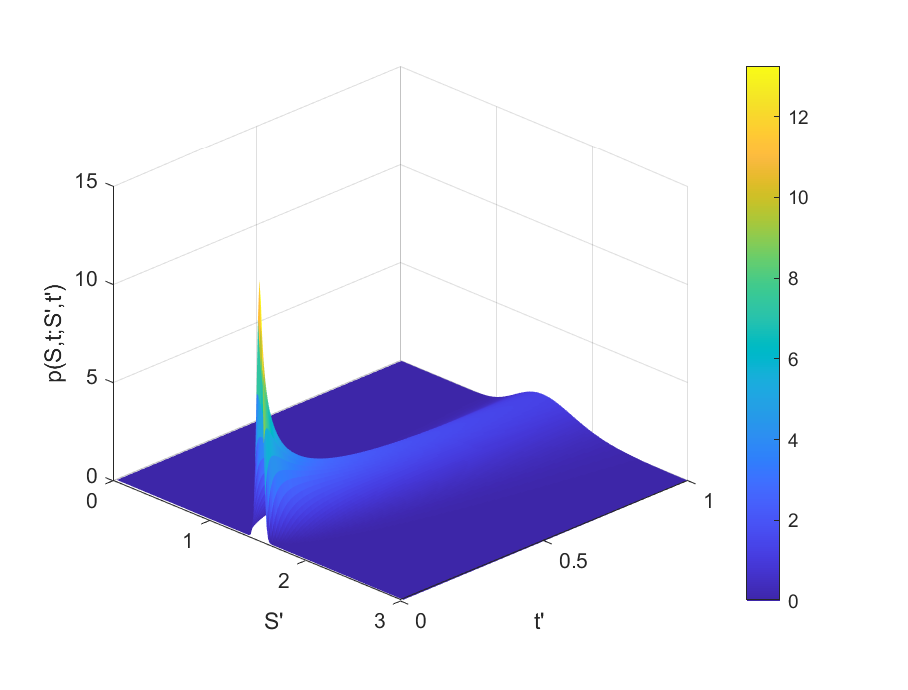
\includegraphics[width=\linewidth]{Imagenes/Parte1/3_Aleatoriedad/PDF_3D.eps}
    \end{subfigure}
        \begin{subfigure}[b]{0.45\linewidth}
        \includegraphics[width=\linewidth]{Imagenes/Parte1/3_Aleatoriedad/PDF_2D.eps}
    \end{subfigure}
    \caption{Función de densidad de transición}
\end{figure}



\subsubsection{Ecuación de Kolmogorov hacia detrás}
Se centra en cómo evoluciona la densidad de transición con respecto al tiempo actual $t$. Se enfoca más en el origen  y cómo cambian las probabilidades de llegar al punto $y'$, $t'$ dependiendo de donde se está en el momento. La EDP es
\[
    \boxed{\frac{\partial p}{\partial t} + \frac{1}{2} B(y, t)^2 \frac{\partial^2 p}{\partial y^2} + A(y, t) \frac{\partial p}{\partial y} = 0}
\]


\subsubsection{Distribución en estado estacionario (steady-state distribution)}
Son aquellas cuya función de densidad de transición $p(y, t; y', t')$ tiende, cuando $t' \to \infty$, a una distribución que ya no depende del estado inicial $y$ ni del tiempo $t$. Para eso se debe cumplir que el proceso sea homogéneo en el tiempo, i.e. $A$ y $B$ sean independientes de $t$ en el límite asintótico. Cuando se cumple la función de densidad de transición converge a $p_\infty(y')$ que satisface:
\[
    \boxed{\frac{1}{2} \frac{d^2}{dy'^2} \left( B_\infty^2 p_\infty \right) - \frac{d}{dy'} \left( A_\infty p_\infty \right) = 0}
\]
donde $A_\infty$ y $B_\infty$ son los valores de los coeficientes en el límite $t \to \infty$.








\section{Tiempos de primer escape (First-exit times)}\label{sec:FirstExitTimes}
El \textit{first-exit time} es el tiempo en el cual un camino aleatorio alcanza un cierto límite por primera vez. El objetivo de esta sección es calcular la probabilidad de que un camino aleatorio alcance cierto límite antes de cierto tiempo.
\begin{figure}[H]
    \centering
    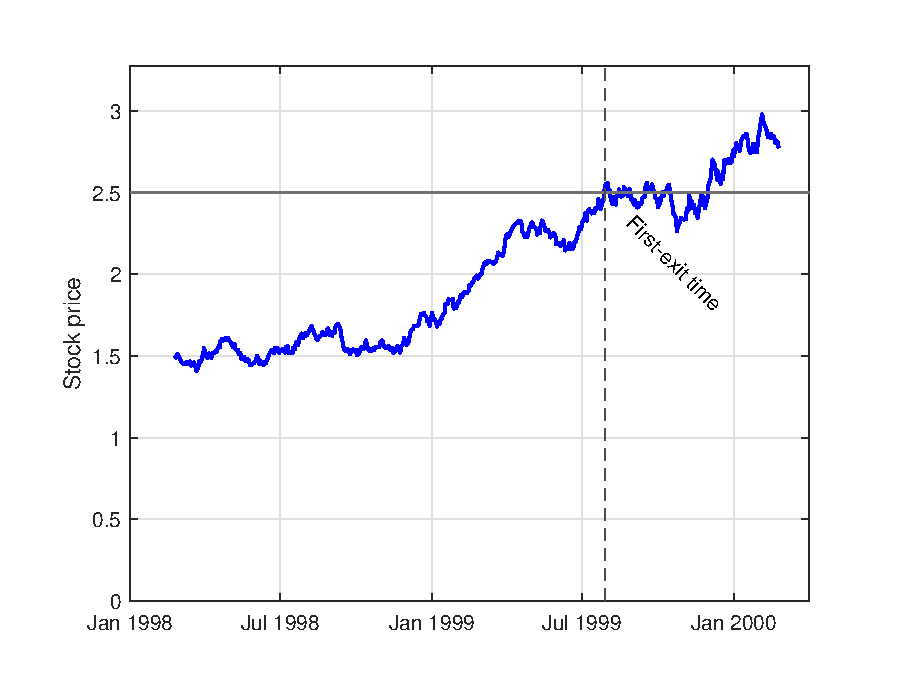
\includegraphics[width=0.65\linewidth]{Imagenes/Parte1/3_Aleatoriedad/First-exit_Time.eps}
    \caption{First-exit Time}
\end{figure}




\subsection{Funciones de distribución acumulada para first-exit times}
Se definde la función $C(y, t; t')$ como la probabilidad de que la variable $y$ salga de la región $\Omega$ antes del tiempo $t'$, habiendo empezado en $y$ en el tiempo $t$. Esta función puede interpretarse como una función de distribución acumulada para first-exit time. 

El objetivo es calcular la probabilidad de que un camino aleatorio abandone una región $\Omega$ antes de un tiempo dado $t'$. Para ello, se tiene que satisfacer el problema de la EDP hacia atrás:
\begin{equation}\label{eq:CumulatFirstExitTime}
    \boxed{
    \left\{
    \begin{array}{rlrl}
        \displaystyle\frac{\partial C}{\partial t} + \frac{1}{2} B(y, t)^2 \frac{\partial^2 C}{\partial y^2} + A(y, t) \frac{\partial C}{\partial y} = 0 &\quad& (y,t) \in \Omega\times(0, t') \\[2ex]
        C(y, t; t') = 1 && (y,t) \in \partial\Omega\times(0, t') \\[2ex]
        C(y, t'; t') = 0 && y \in \Omega \\
    \end{array}
    \right\}
    }
\end{equation}




\subsection{Tiempos de primer escape esperados (Expected first-exit times)}\label{sec:ExpectedFirstExitTimes}
Una vez calculado~\eqref{eq:CumulatFirstExitTime} es posile calcular el tiempo esperado de primer escape:
\[
    u(y, t) = \int_t^\infty (t' - t) \frac{\partial C}{\partial t'} dt' \overset{\text{partes}}{=} \int_t^\infty 1 - C(y, t; t') dt'
\]
por lo tanto,
\begin{align*}
    \frac{\partial u}{\partial t}  &= \frac{\partial}{\partial t} \left(\int_t^\infty 1 - C(y, t; t') dt' \right) \overset{\text{Leibniz}}{=} -\left(1-C(y, t, t)\right) + \int_t^\infty \frac{\partial}{\partial t}\left(1 - C(y, t; t')\right) dt' \\
    &\overset{\text{\eqref{eq:CumulatFirstExitTime}}}{=} -1 - \int_t^\infty \frac{\partial}{\partial t} C(y, t; t') dt' \\
    \frac{\partial u}{\partial y}  &= \int_t^\infty \frac{\partial}{\partial y}\left(1 - C(y, t; t')\right) dt' = - \int_t^\infty \frac{\partial}{\partial y} C(y, t; t') dt' \\
    \frac{\partial^2 u}{\partial y^2}  &= - \int_t^\infty \frac{\partial^2}{\partial y^2} C(y, t; t') dt' \\
\end{align*}
que volviendo a la EDP~\eqref{eq:CumulatFirstExitTime}:
\begin{align*}
    &\int_t^\infty\frac{\partial C}{\partial t} + \frac{1}{2} B(y, t)^2 \frac{\partial^2 C}{\partial y^2} + A(y, t) \frac{\partial C}{\partial y} dt' = 0 \Rightarrow \\
    &\Rightarrow \int_t^\infty\frac{\partial C}{\partial t} dt' + \frac{1}{2} B(y, t)^2 \int_t^\infty \frac{\partial^2 C}{\partial y^2} dt' + A(y, t) \int_t^\infty \frac{\partial C}{\partial y} dt' = 0 \Rightarrow \\
    &\Rightarrow -1 - \frac{\partial u}{\partial t} - \frac{1}{2} B(y, t)^2 \frac{\partial^2 u}{\partial y^2} - A(y, t) \frac{\partial u}{\partial y} = 0
\end{align*}
por lo que el tiempo esperado de primer escape $u(y, t)$ satisface la EDP
\[
    \boxed{
        \left\{
        \begin{aligned}
            \frac{\partial u}{\partial t} + \frac{1}{2} B(y, t)^2 \frac{\partial^2 u}{\partial y^2} + A(y, t) \frac{\partial u}{\partial y} = -1\\
            u(y, t) = 0 && y \in \partial\Omega \\
        \end{aligned}
        \right\}
    }
\]
Por ejemplo, si se tiene una EDE independiente del tiempo $A=\mu S, B=\sigma S$, se puede buscar una solución en estado estacionario, es decir, $u(y, t) = u(y)$, que satisface la EDP
\[
    \frac{1}{2}\sigma^2 S^2 \frac{d^2 u}{dS^2} + \mu S \frac{du}{dS} = -1
\]
con condiciones de contorno $u(S_0) = u(S_1) = 0$. La solución en este caso sería.
\[
    u(S) = \frac{1}{\frac{1}{2}\sigma^2 - \mu} \left( \log(S/S_0) - \frac{1 - (S/S_0)^{1-2\mu/\sigma^2}}{1 - (S_1/S_0)^{1-2\mu/\sigma^2}} \log(S_1/S_0) \right)
\]








\section{Estrategias en apuestas}

\subsection{Blackjack}
La distribución del beneficio en el blackjack (explicado en el apéndice~\ref{sec:blackjack}) es la siguiente. Se denota $\phi$ a la variable aleatoria que represestan el resultado de la apuesta, $\mu$ es la media de y $\sigma$ es la desviación típica de $\phi$. En blackjack, los valores discretos de $\phi$ son:
\begin{align*}
    &\phi = -1, && \text{el jugador pierde la apuesta} \\
    &\phi = 0, && \text{el jugador empata} \\
    &\phi = 1, && \text{el jugador gana la apuesta} \\
    &\phi = 3/2, && \text{el jugador consigue un blackjack o natural} \\
\end{align*}
\begin{figure}[H]
    \centering
    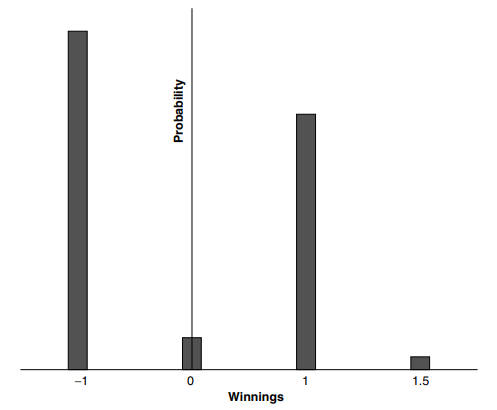
\includegraphics[width=0.65\linewidth]{Imagenes/Parte1/3_Aleatoriedad/blackjack_Dist.png}
    \caption{Distribución de beneficios en el blackjack}
\end{figure}




\subsection{Criterio de Kelly}
Siguiendo con el ejemplo del blackjack, se tiene la v.a.\ $\phi_i$ para denotar el resultado de mano i-ésima, con media $\mu_i$ y desviación típica $\sigma_i$. Suponiendo además que en total incialmente se tiene una cantidad de dinero $P$ y en cada mano se apuesta una fracción $f$ de la cantidad de dinero que se tenga en ese momento. Por lo tanto en la primera mano se obtiene
\[
    P(1+f\phi_1)
\]
en la segunda mano
\[
    P(1+f\phi_1)(1+f\phi_2)
\]
y tras $M$ manos se obtiene
\[
    P\prod_{i=1}^M (1+f\phi_i)
\]
se plantea ahora cómo se elige $f$ para maximiar las ganancias. Si $f$ es muy grande eventualmente se perderá todo (o casi todo el dinero) aunque las expectativas sean positivas (por ejemplo, si se apuesta todo el dinero en una mano); si $f$ es muy es muy pequeño, se ganrá poco y se tardará demasiado en conseguir una cantidad significativa de dinero. Por lo tanto se  busca un valor intermedio.

En este caso se va a elegir $f$ de forma que maximice la \textbf{tasa de crecimiento esperada a largo plazo}, si bien se pueden maximizar con otras estrategias. La tasa de crecimiento es
\[
    \frac{1}{M} \ln\left(  P\prod_{i=1}^M (1+f\phi_i)\right) = \frac{1}{M} \ln(P) + \frac{1}{M} \sum_{i=1}^M \ln(1+f\phi_i)
\]
ignorando el reescalado del primer término y suponiendo que el resultado de cada mano es independiente (no es el caso en el blackjack), su esperanza es:
\begin{align*}
    \mathbb{E}[\ln(1+f\phi_i)] &\overset{\text{(Taylor)}}{=} \mathbb{E}[f\phi_i - \frac{1}{2}f^2\phi_i^2 + O(f^3)] \\
    &= f\mathbb{E}[\phi_i] - \frac{1}{2}f^2\mathbb{E}[\phi_i^2] + O(f^3) \\
    &= f\mu - \frac{1}{2}f^2\sigma^2 + O(f^3)
\end{align*}

Luego, despreciando los términos de orden superior, la tasa de crecimiento esperada a largo plazo es
\begin{align}\label{eq:KellyGrowth}
    f\mu - \frac{1}{2}f^2\sigma^2
\end{align}
que se maximiza cuando
\[
    \boxed{f = \frac{\mu}{\sigma^2}}
\]
dando un crecimiento esperado de
\[
    \frac{\mu}{\sigma^2}\mu - \frac{1}{2}\left(\frac{\mu}{\sigma^2}\right)^2\sigma^2 = \frac{\mu^2}{\sigma^2} - \frac{1}{2}\frac{\mu^2}{\sigma^2} = \boxed{\frac{\mu^2}{2\sigma^2}}
\]
por mano.

Lo importante para obtener ganancias a largo plazo es que la ecuación~\eqref{eq:KellyGrowth} sea positiva:
\begin{align*}
    f\mu - \frac{1}{2}f^2\sigma^2 > 0 \Leftrightarrow f\mu > \frac{1}{2}f^2\sigma^2 \Leftrightarrow \mu > \frac{1}{2}f\sigma^2 \Leftrightarrow \boxed{f < \frac{2\mu}{\sigma^2}}
\end{align*}







\subsection{Apuestas a eventos deportivos: carreras de caballos}
Se tiene en una carrera de caballos $N$ caballos, habiendose apostado una cantidad total $W_i$ sobre el i-ésimo caballo. La casa de apuestas paga $1:q_i$ por el iésimo caballo. Para evitar pérdidas, la casa de apuestas tiene que elegir $q_i$ de forma que nunca pierda.

El total de dinero recaudado antes de la carrera es de
\[
    \sum_{i=1}^N W_i
\]
y si el gana el caballo $j$ la casa de apuestas paga 
\[
    (1+q_j)W_j
\]
luego para conseguir ganancias, lo único de lo que tiene que asegurarse la casa de apuestas es de que
\[
    \sum_{i=1}^N W_i \geq (1+q_j)W_j
\]
es decir que
\[
    \boxed{q_j \leq \frac{\sum_{i=1}^N W_i}{W_j} - 1, \quad \forall j=1,\ldots,N}
\]

Como se puede observar, la probabilidades no tienen nada que ver con las probabilidades reales, si no de lo que se haya apostado.





Ahora desde el punto de vista del apostador, veamos si se puede observar si hay arbitraje. Sea $w_i$ la cantidad apostada al i-ésimo caballo y que el total de dinero apostado es 1, entonces
\[
    \sum_{i=1}^N w_i = 1
\]
y lo que se gana siendo el j-ésimo caballo el ganador es
\[
    (q_j + 1)w_j
\]

El objetivo es por lo tanto encontrar $w_i$ para todo i tal que son todos positivos, suman 1 y la ganancia sea postivia para todo $j$. Por lo tanto, para que haya arbitraje se tiene que conseguir más de 1 (lo invertido):
\begin{align*}
    (q_j + 1)w_j > 1 \Leftrightarrow w_j > \frac{1}{q_j + 1} \\
\end{align*}
leugo el problema es encontrar $w_i$ tal que
\[
    \left\{
    \begin{aligned}\label{eq:ArbitrajeCaballos}
        &\sum_{i=1}^N w_i = 1 \\
        &w_j > \frac{1}{q_j + 1} \quad \forall j
    \end{aligned}
    \right\}
\]
La primera parte implica que la solución debe estar en en plano $\sum_{i=1}^N w_i = 1$ mientras que la segunda dice que para que haya arbitraje el punto $\frac{1}{\vec{q} + 1}$ debe estar por debajo de dicho plano, teniendo en cuenta que todos los valores deben ser positivos. En 2D esto se traduce en la siguiente imagen:
\begin{figure}[H]
    \centering
    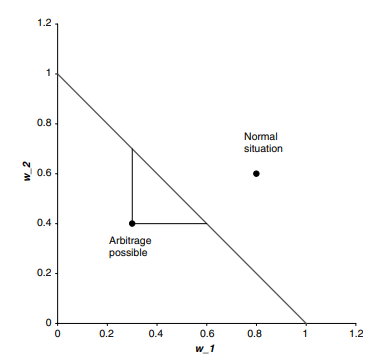
\includegraphics[width=0.65\linewidth]{Imagenes/Parte1/3_Aleatoriedad/Arbitraje_Cabllos.png}
    \caption{Arbitraje en carreras de caballos de dos caballos}
\end{figure}

Una manera rápida de comprobar si hay arbitraje es transformar la ecuacion~\eqref{eq:ArbitrajeCaballos} y comprobar si se cumple:
\[
    1 = \sum_{i=1}^N w_i > \sum_{i=1}^N \frac{1}{q_i + 1} \Rightarrow  \boxed{\sum_{i=1}^N \frac{1}{q_i + 1} < 1}
\]
en caso contrario no hay arbitraje. Una vez comprobado que hay arbitraje, para conseguir ganancias simplemente se debe conseguir un punto $\vec{w}$ dentro de la recta (o plano) $\sum_{i=1}^N w_i = 1$ (comprobando que se cumple la otra condición).





Si no se cumple la condición de arbitraje, existen varias maneras de apostar. Sea $p_i$ la probabilidad de que el i-ésimo caballo gane, entonces se debe cumplir.
\[
    \sum_{i=1}^N p_i = 1
\]
Si se ha apostado en todos los caballos un total de 1, entonces el beneficio o pérdida esperado es
\[
    m = \sum_{i=1}^N p_i w_i (q_i + 1) - 1
\]

Por otro lado, la desviación estandar es
\[
    \sigma = \sqrt{\sum_{i=1}^N p_i( w_i (q_i + 1) - 1 - m)^2}
\]

Existen varias estrategias de apuestas:
\begin{itemize}
    \item \textbf{Maximizar el valor esperado}: en este caso se apuesta todo al caballo con mayor probabilidad de ganar, i.e.\ maximizar $p_i(q_i+1)$. Esta es una apuesta muy arriesgada ya que la esperanza es muy alta pero también la desviación.
    \item \textbf{Minimizar la desviación estándar}: muchas veces se consigue una desviación nula, pero resulta en una esperanza negativa, por lo que no es una buena estrategia.
    \item \textbf{Maximizar rendimiento dividido por desviación estándar}: en este caso se busca un equilibrio entre la esperanza y la desviación $m/\sigma$.
\end{itemize}













\section{Extreme value theory}
Estudia el comportamiento de los valores extremos de una variable aleatoria, es decir, los máximos y mínimos. Se centra en la distribución de los valores extremos, que normalmente con pocas observaciones.

Si $X_i$ son variable identicamente distribuidas (iid) y
\[
    x = \max(X_1, X_2, \ldots, X_n)
\]
entonces la función de distribución de $x$ converge a
\[
    \boxed{F(x) = \exp\left( -\left( 1 + \frac{\xi (x-\mu)}{\sigma} \right)^{-1/\xi} \right)}
\]
donde si $\xi=0$ se tiene la distribución Gumbel, si $\xi > 0$ se tiene la distribución Fréchet y si $\xi < 0$ se tiene la distribución Weibull. En concreto, la de Fréchet es importante en finanzas porque esta asociada a colas pesadas.


Se considera la probabilidad de una pérdida que exceda $u$ por una cantidad $y$, sabiendo que se ha superado $u$, es decir,
\[
    F_u(x) = \mathbb{P}(X - u \leq  y \mid X > u)
\]
Esto se puede aproximar por la Distribución Generalizada de Pareto (GPD):
\[
    \boxed{1 - \left( 1 + \frac{\xi X}{\beta} \right)^{-1/\xi}}
\]

Para colas pesadas, se tiene que $\xi > 0$, en cuyo caso no todos los momentos existen:
\[
    \mathbb{E}[X^k] = \infty, \qquad k \geq \frac{1}{\xi}
\]

Para más información mirar teoría vista en el Athens.





